\documentclass[11pt]{article}
\usepackage[margin=1in]{geometry}
\usepackage{amsmath,amssymb,amsthm,mathtools}
\usepackage{enumitem,booktabs,longtable}
\usepackage{pgfplots}
\pgfplotsset{compat=1.18}
\usetikzlibrary{pgfplots.groupplots}
\allowdisplaybreaks[2]
\usepackage{xurl}
\usepackage[hidelinks]{hyperref}
\hypersetup{pdftitle={Removing the logarithmic loss in the Li-Wu KdV integrator},pdfauthor={Kaiwen Jin}}
\usepackage[T1]{fontenc}
\usepackage{lmodern,microtype}
\newtheorem{theorem}{Theorem}
\newtheorem{lemma}[theorem]{Lemma}
\newtheorem{proposition}[theorem]{Proposition}
\newtheorem{corollary}[theorem]{Corollary}
\theoremstyle{remark}\newtheorem{remark}[theorem]{Remark}
\newcommand{\T}{\mathbb T}
\newcommand{\Z}{\mathbb Z}
\newcommand{\R}{\mathbb R}
\newcommand{\cR}{\mathcal R}
\newcommand{\cC}{\mathcal C}
\newcommand{\cJ}{\mathcal J}
\newcommand{\cB}{\mathcal B}
\newcommand{\norm}[2][]{\left\lVert #2\right\rVert_{#1}}
\newcommand{\abs}[1]{\left|#1\right|}
\newcommand{\ip}{\partial_x^{-1}}
\newcommand{\supp}{\operatorname{supp}}
\newcommand{\sinc}{\operatorname{sinc}}
\newcommand{\esssup}{\operatorname*{ess\,sup}}
\title{Removing the logarithmic loss in the Li--Wu KdV integrator}
\author{Kaiwen Jin\\\texttt{yui.ui.siki@gmail.com}}
\date{10 October 2026}

\begin{document}
\maketitle
\begin{abstract}
Li and Wu proved that their unfiltered integrator for periodic KdV converges
in $L^2$ with error $O(\tau^\gamma\log(1/\tau))$ for real, mean-zero
$H^\gamma$ data, $0<\gamma\leq1$. We remove the logarithmic factor for the
same time-semidiscrete algorithm, with constants uniform on bounded
$H^\gamma$ sets. The main estimate concerns the exact averaged cubic
remainder. Retaining both ratios of its two oscillatory phases bounds the
dual four-frequency multiplier by the reciprocal of the third largest
frequency. A dyadic four-linear estimate sums this majorant without a
logarithm and includes a mixed $L^2$ endpoint. That endpoint controls the
remainder at the numerical state without a numerical Sobolev bound.
We then prove the full global estimate using the continuous trilinear
bounds of Li and Wu, a stepwise residual calculation, low--high frequency
stability, a restarted bootstrap, and density. Finite Fourier experiments
check the implemented update, the remainder, and accumulated step defects.
\end{abstract}

\section{Introduction}
Low spatial regularity limits the accuracy of time discretizations for
dispersive equations. For periodic KdV, differentiation in the quadratic
nonlinearity makes a direct $L^2$ perturbation estimate insufficient.
The unfiltered method of Li and Wu integrates the leading oscillatory
interactions explicitly and treats its numerical trajectory as a perturbed
KdV solution. Their convergence theorem gives
$C\tau^\gamma\log(1/\tau)$ in $L^2$ for $H^\gamma$ data with
$0<\gamma\leq1$ \cite[Theorem~1.1]{LW}.
The necessity of the logarithm is left open in
\cite[Section~11]{LW}; this is the fixed-scheme question in
AIM problem~518 \cite{AIM}.

We prove the bound $C\tau^\gamma$ for that same method, uniformly on bounded
sets of real, mean-zero $H^\gamma$ data. The improvement comes from the
averaging remainder, rather than a change in the update. Its multiplier
contains the covariance of two exponential phases. Each phase can be
integrated against the other, giving two ratio bounds. Keeping their
minimum matters when the output frequency is small. After duality the four
frequencies sum to zero, their largest two magnitudes are comparable, and
the remaining multiplier is controlled by $1/N_3$, where $N_3$ is the
third largest magnitude. The smaller dyadic scales then carry a summable
geometric factor.

The resulting trilinear estimate includes exponent zero. This is a local
remainder estimate: it does not assert a uniform global rate on an $L^2$
ball. Its role is to compare the cubic remainder at the numerical state
with the remainder at an exact $H^\gamma$ state using only their $L^2$
difference. We retain the continuous trilinear estimates of Li and Wu
and give the residual and stability argument in full. In particular,
the normal-form identity keeps both endpoints when the time interval is
restarted, and its forcing term is estimated from the actual stepwise
residual. A fixed-timestep approximation argument then removes the
temporary smoothness used in the calculations.

The experiments use a fixed finite Fourier cutoff, complete polynomial
intermediates, and independently checked reference resolutions. They
illustrate the remainder and error accumulation. Every computed input is
a smooth Fourier polynomial, so these observations do not decide a
uniform rough-data rate or the necessity of a logarithm; that conclusion
is proved analytically below.
\section{The scheme and the main result}
Use normalized measure $dx/(2\pi)$ on $\T=\R/(2\pi\Z)$; changing to unnormalized
$L^2$ only changes constants. Write $S_t=e^{-t\partial_x^3}$, so that
$\widehat{S_tf}(k)=e^{itk^3}\widehat f(k)$.
Let $P_0$ be the mean, $P=I-P_0$, and define $D^{-1}=\ip$ with multiplier
$(ik)^{-1}$ for $k\ne0$ and zero at zero. Set $D^{-2}=(D^{-1})^2$.
Write $\widehat f(k)=(2\pi)^{-1}\int_0^{2\pi}f(x)e^{-ikx}\,dx$ and
$\|f\|_{H^s}^2=\sum_{k\in\Z}\langle k\rangle^{2s}|\widehat f(k)|^2$,
$\langle k\rangle=(1+k^2)^{1/2}$. Spaces are the completions of trigonometric
polynomials in these norms, with negative spaces interpreted as distributions.
Orthogonality gives the normalized $L^2$ identity for polynomials and hence
for their completions. For mean-zero functions and $s\geq0$,
$\|f\|_{\dot H^s}\leq\|f\|_{H^s}\leq2^{s/2}\|f\|_{\dot H^s}$;
For $s<0$, $2^{s/2}\|f\|_{\dot H^s}\leq\|f\|_{H^s}\leq\|f\|_{\dot H^s}$.
Real-valued means $\widehat f(-k)=\overline{\widehat f(k)}$.
All time suprema concern continuous representatives; derivative norms are
essential suprema. The exact solution is the unique real mean-zero
$C([0,T];H^\gamma)$ solution obtained by smooth approximation, and satisfies
the equation distributionally. The constants $C_M$ may change from line to line and depend on
$\gamma,T,M$, but are uniform in $n,\tau$ and spectral support.


The equation is
\begin{equation}\label{eq:kdv}
u_t+u_{xxx}=\tfrac12\partial_x(u^2),\qquad u(0)=u_0.
\end{equation}
The fixed scheme is $u^0=u_0$ and
\begin{equation}\label{eq:scheme}
u^{n+1}=S_\tau u^n+F_\tau(u^n)+H_\tau(u^n),\qquad \tau=T/L,
\end{equation}
where
\begin{align*}
F_\tau(f)&=\tfrac16P[(S_\tau D^{-1}f)^2]-\tfrac16S_\tau P[(D^{-1}f)^2],\\
H_\tau(f)&=\tfrac13P[(S_\tau D^{-1}f)D^{-1}F_\tau(f)]
 +\tfrac\tau9(S_\tau D^{-1}f)P_0(f^2)\\
&\quad-\tfrac1{54}\left[S_{\tau-s}D^{-1}[(S_sD^{-1}f)^3]\right]_{s=0}^{s=\tau}\\
&\quad-\tfrac1{27\tau}\left[S_{\tau-s}D^{-2}
 [(S_{s-\tau}D^{-2}F_\tau(f))(S_sD^{-1}f)]\right]_{s=0}^{s=\tau}.
\end{align*}
This is the scheme of \cite[Eq.~(1.4)]{LW}, without a spatial frequency cutoff.

\begin{theorem}[Logarithm-free convergence]\label{thm:main}
Let $T>0$, $0<\gamma\leq1$, and $R>0$. For real, mean-zero
$u_0\in H^\gamma(\T)$ with $\norm[H^\gamma]{u_0}\leq R$, there are
$C,\tau_0>0$, depending only on $T,\gamma,R$, such that the scheme
\eqref{eq:scheme} satisfies
\[
\max_{0\leq n\leq L}\norm[L^2]{u(n\tau)-u^n}\leq C\tau^\gamma
\quad\text{whenever }\tau=T/L\leq\tau_0.
\]
\end{theorem}
The periodic KdV bounds of Babin--Ilyin--Titi control the exact flow on
the initial-data ball. The continuous estimates of
\cite[Proposition~3.4 and Lemma~7.2]{LW} will be used in the stability proof.
The logarithmic convergence theorem itself is not used.
For the exact twisted solution $v(t)=S_{-t}u(t)$, set
\[
M=1+\sup_{0\leq t\leq T}\norm[H^\gamma]{v(t)}.
\]
The source statements and the sign transformation giving a bound for $M$
are recorded below in Section~\ref{sec:flow}. No convergence theorem for the
numerical scheme is used as an input. Intermediate constants may depend on $M,\gamma,T$,
but never on the timestep or a Fourier support bound.

\subsection{The exact KdV flow}\label{sec:flow}
The source \cite[Theorems~4.2--4.3, 5.1, 6.3--6.5]{BIT} treats
$U_t=UU_x+U_{xxx}$ on the same torus, with normalized measure and
mean-zero homogeneous Sobolev norms. Theorem~4.2 bounds its Galerkin flows
on $[0,T]$ in $\dot H^s$ by a constant depending only on
$s,T,\|U_0\|_{\dot H^s}$ and an upper bound for $\|U_0\|_2$.
Theorem~4.3 gives a distributional limiting solution with the same bound.
Theorems~5.1 ($s>1/2$) and 6.3 ($0<s\leq1/2$) give its uniqueness,
$C([0,T];\dot H^s)$ regularity and continuous dependence. Theorem~6.4
covers $s=0$, and Theorem~6.5 with $\theta=0$ states that, for two flows
whose initial $L^2$ norms sum to at most $B$,
$\sup_{[0,T]}\|U-\widetilde U\|_2\leq C(T,B)\|U_0-\widetilde U_0\|_2$.
Together these results specify the continuous flow and the uniform
bounds needed here.

Define $u(t,x)=-U(t,-x)$. Then
$u_t=-U_t$, $u_x=U_x$, $u_{xxx}=U_{xxx}$ at $(t,-x)$, and consequently
$u_t+u_{xxx}=uu_x$. Fourier coefficients become
$\widehat u(k)=-\widehat U(-k)$, preserving every Sobolev norm, reality
and zero mean. This transforms the source equation to \eqref{eq:kdv}.
The norm comparison above transfers all bounds to our $H^\gamma$ norm.
Hence there is $A(T,\gamma,R)<\infty$ such that every smooth
initial datum in the stated ball satisfies
$\sup_{[0,T]}\|u(t)\|_{H^\gamma}\leq A$.
The same bound holds for the limiting solution: for each finite set of
frequencies pass to the limit in its finite norm sum, then take the supremum
over finite sets. Thus $M\leq1+A(T,\gamma,R)$ uniformly. Continuous
dependence in $L^2$ is precisely the input used in the final density passage.
No change of torus length or amplitude scaling is needed.

\section{The averaged cubic remainder}\label{sec:remainder}
The estimate proved in this section is uniform in the Fourier support.
We begin with the exact covariance in the update.
\subsection{Covariance bounds}
For real $\alpha,\beta$ let
\[
M_\tau g=\frac1\tau\int_0^\tau g(s)\,ds,\qquad
\eta_\tau(\alpha,\beta)=M_\tau(e^{-is(\alpha+\beta)})
-M_\tau(e^{-is\alpha})M_\tau(e^{-is\beta}).
\]
For $k=a+b+c$, put
\begin{equation}\label{eq:phases}
p=a+b,\quad \alpha=3abp,\quad \beta=3kcp,\quad
\Phi=\alpha+\beta=k^3-a^3-b^3-c^3.
\end{equation}
In the notation of \cite[Eqs.~(4.15),(6.1)]{LW},
\begin{equation}\label{eq:R2}
\widehat{R_{2,\tau}^{n}(f_1,f_2,f_3)}(k)
=-\frac{\tau}{18ik}\sum_{\substack{a+b+c=k\\a+b\ne0}}
e^{-it_n\Phi}\eta_\tau(\alpha,\beta)
\widehat f_1(a)\widehat f_2(b)\widehat f_3(c),\quad k\ne0,
\end{equation}
with zero output at $k=0$. Terms with a zero input frequency also vanish,
because then $\alpha=0$ or $\beta=0$.

\begin{lemma}[Bounds for the average covariance]\label{lem:eta}
If $\alpha\beta\ne0$, then
\begin{align}
\abs{\eta_\tau(\alpha,\beta)}&\leq2\min\{\abs{\alpha/\beta},\abs{\beta/\alpha}\},\label{eq:ratio}\\
\abs{\eta_\tau(\alpha,\beta)}&\leq\tau\min\{\abs\alpha,\abs\beta\}.\label{eq:smalltime}
\end{align}
If either phase vanishes, $\eta_\tau=0$.
\end{lemma}
\begin{proof}
Let $h(s)=e^{-i\alpha s}-M_\tau(e^{-i\alpha s})$. Then
$\eta_\tau=\tau^{-1}\int_0^\tau h(s)e^{-i\beta s}\,ds$.
The elementary bound
$\abs{h(s)}\leq\tau^{-1}\int_0^\tau\abs\alpha\abs{s-r}\,dr
\leq\tau\abs\alpha$ gives \eqref{eq:smalltime}, also interchanging
$\alpha$ and $\beta$. Moreover,
\[
\abs{h(0)}+\abs{h(\tau)}\leq\tau\abs\alpha,
\qquad \int_0^\tau\abs{h'(s)}\,ds=\tau\abs\alpha.
\]
Integrating $e^{-i\beta s}$ once gives
$\abs{\eta_\tau}\leq2\abs{\alpha/\beta}$.
Interchanging the phases proves \eqref{eq:ratio}. These estimates are
consistent with \cite[Lemma~3.2]{LW}; the proof here records exactly which
bounds will be retained.
\end{proof}

\subsection{Four frequencies and dyadic summation}
For nonzero $a,b,c,d\in\Z$ with $a+b+c+d=0$, let
$N_1\geq N_2\geq N_3\geq N_4$ be the decreasing rearrangement of their
absolute values. Thus $N_3$ is the third largest, or second smallest, of
\emph{four} frequencies, including the dual output $d=-k$.
The zero-sum relation implies $N_1\leq3N_2$.

\begin{lemma}[Two pointwise majorants]\label{lem:geometry}
Write $A=\abs{ab}$ and $B=\abs{cd}$. Then
\begin{align}
\frac1{\abs d}\min\{A/B,B/A\}&\leq\frac3{N_3},\label{eq:m0}\\
\frac{\abs{a+b}}{\max(A,B)}&\leq\frac6{N_3}.\label{eq:m1}
\end{align}
\end{lemma}
\begin{proof}
For \eqref{eq:m0}, if $d$ is among the two largest frequencies, use
$\min(A/B,B/A)\leq1$. Otherwise the largest two are among $a,b,c$.
If they are $a,b$, then
\[
\frac1{\abs d}\min(A/B,B/A)\leq\frac{\abs c}{\abs{ab}}
\leq\frac1{N_3}.
\]
If they are $a,c$ (the case $b,c$ is identical), their ratio is between
$1/3$ and $3$. The remaining magnitudes are $\abs b,\abs d$, whose maximum is
$N_3$. Thus
\[
\frac1{\abs d}\min(A/B,B/A)
\leq3\min\left\{\frac{\abs b}{\abs d^2},\frac1{\abs b}\right\}
\leq\frac3{\max(\abs b,\abs d)}.
\]
For \eqref{eq:m1}, consider the pairing $(a,b)$ and $(c,d)$.
If the two largest magnitudes are in the same pair, the other pair has
sum of magnitude at most $2N_3$. Since $a+b=-(c+d)$,
\[
\frac{\abs{a+b}}{\max(A,B)}\leq\frac{2N_3}{N_1N_2}\leq\frac2{N_3}.
\]
If the largest two belong to different pairs, the third largest is paired
with one of them. Hence $\max(A,B)\geq N_2N_3$ and
$\abs{a+b}\leq2N_1\leq6N_2$, giving the result.
Ties can be ordered arbitrarily; the same alternatives cover them.
\end{proof}

\begin{lemma}[Third-largest-frequency four-linear estimate]\label{lem:fourlinear}
For nonnegative $x_j\in\ell^2(\Z\setminus\{0\})$,
\begin{equation}\label{eq:fourlinear}
\sum_{\substack{a+b+c+d=0\\abcd\ne0}}
\frac{x_1(a)x_2(b)x_3(c)x_4(d)}{N_3(a,b,c,d)}
\leq C\prod_{j=1}^4\norm[\ell^2]{x_j}.
\end{equation}
The same conclusion holds after restricting the sum to any subset.
\end{lemma}
\begin{proof}
It suffices first to consider finitely supported sequences. Decompose into
shells $2^j\leq\abs k<2^{j+1}$, $j\geq0$, and write $X_{r,j}$ for the
$\ell^2$ norm of the $r$th sequence on the $j$th shell. Fix an ordering
of the four shell indices $j_1\geq j_2\geq j_3\geq j_4$.
A nonzero zero-sum interaction has $j_1-j_2\leq2$.
For each fixed pair of smaller-shell frequencies, the remaining sum of the
two larger-shell sequences is at most their $\ell^2$ norm product by
Cauchy--Schwarz, since one sequence is a translated reflection of the other.
Sum the smaller frequencies in $\ell^1$. A shell has at most $2^{j+1}$
integer elements, so another Cauchy--Schwarz bound gives
\[
\sum_{a+b+c+d=0}\prod_{r=1}^4 x_{r,j_r}
\leq C2^{(j_3+j_4)/2}\prod_{r=1}^4X_{r,j_r}.
\]
Since $N_3\geq2^{j_3}$, the weight leaves
$C2^{-(j_3-j_4)/2}$. For $q=j_1-j_2\in\{0,1,2\}$, extend the nonnegative
sum by dropping the upper restriction on the smaller shells. The contribution
is at most
\[
C\left(\sum_JX_{1,J}X_{2,J-q}\right)
\left(\sum_{\ell\geq m}2^{-(\ell-m)/2}X_{3,\ell}X_{4,m}\right).
\]
The first factor is bounded by Cauchy--Schwarz. Writing $r=\ell-m$, the second
is at most
\[
\sum_{r\geq0}2^{-r/2}\norm[\ell^2]{X_3}\norm[\ell^2]{X_4}
=\frac{\norm[\ell^2]{X_3}\norm[\ell^2]{X_4}}{1-2^{-1/2}}.
\]
Sum over at most 24 orderings and three offsets. For arbitrary nonnegative
sequences apply the finite bound to their restrictions to $|k|\leq m$.
The infinite positive sum is the supremum of these finite sums, while the
norms of the restrictions are bounded by the full norms. This proves the
infinite statement without exchanging conditionally convergent sums.
\end{proof}

\subsection{The mixed remainder estimate}
\begin{theorem}[Mixed remainder bound]\label{thm:local}
For $0\leq\gamma\leq1$, $\tau>0$, and arbitrary mean-zero inputs
$f_j\in H^\gamma(\T)$,
\begin{equation}\label{eq:local}
\norm[L^2]{R_{2,\tau}^{n}(f_1,f_2,f_3)}
\leq C\tau^{1+\gamma}\prod_{j=1}^3\norm[H^\gamma]{f_j},
\end{equation}
uniformly in $n$, $\tau$, and Fourier support. The estimate remains true
if an arbitrary multiplier of modulus at most one is inserted in the sum
\eqref{eq:R2}. In particular it holds separately on $\Phi=0$ and $\Phi\ne0$.
\end{theorem}
\begin{proof}
Only nonzero $abck$ and $p=a+b\ne0$ need consideration. Set $d=-k$.
Lemma~\ref{lem:eta} and \eqref{eq:m0} give
\[
\frac{\abs\eta}{\abs k}\leq\frac6{N_3}.
\]
For the other endpoint, observe that $AB=\abs{abck}$, and use
\eqref{eq:smalltime} and \eqref{eq:m1}:
\[
\frac{\abs\eta}{\tau\abs{abck}}
\leq3\frac{\abs p\min(A,B)}{AB}
=3\frac{\abs p}{\max(A,B)}\leq\frac{18}{N_3}.
\]
Taking the geometric mean of these two bounds yields
\begin{equation}\label{eq:central}
\boxed{\quad
\frac{\abs{\eta_\tau(\alpha,\beta)}}{\abs k\,\abs{abc}^{\gamma}}
\leq\frac{6^{1-\gamma}18^\gamma\tau^\gamma}{N_3(a,b,c,-k)}.
\quad}
\end{equation}
Dualize \eqref{eq:R2} against an $\ell^2$ sequence and take absolute values.
Apply Lemma~\ref{lem:fourlinear} with
$x_1(a)=\abs a^\gamma\abs{\widehat f_1(a)}$ and analogously for $x_2,x_3$;
$x_4(d)$ is the absolute value of the dual coefficient at $-d$.
Their norms are bounded by the inhomogeneous Sobolev norms and the dual norm.
The factors $e^{-it_n\Phi}$ have modulus one. This proves the theorem,
including the assertion about restricted sums. Polynomial approximation
and the bound extend the operator to the claimed spaces.
\end{proof}

\begin{remark}
The exponent-zero assertion above is an estimate for the local cubic remainder,
not a convergence theorem at $\gamma=0$. The global closure below uses $\gamma>0$.
\end{remark}

\begin{corollary}[A numerical-state estimate]\label{cor:numerical}
Let $w\in H^\gamma$, $f\in L^2$, $\norm[H^\gamma]{w}\leq M$ and
$\delta=\norm[L^2]{f-w}\leq1$. For $0<\tau\leq1$,
\begin{equation}\label{eq:numerical}
\norm[L^2]{R_{2,\tau}^{n}(f,f,f)}\leq C_M\tau(\tau^\gamma+\delta).
\end{equation}
\end{corollary}
\begin{proof}
Apply \eqref{eq:local} with exponent $\gamma$ to $(w,w,w)$.
Expand the difference between the cubic expressions at $f$ and at $w$,
and apply its exponent-zero case to every difference term. This gives
$C\tau\delta(\norm[L^2]{f}+\norm[L^2]{w})^2$.
No $H^\gamma$ bound on the numerical state is used.
\end{proof}

\section{Global convergence}\label{sec:convergence}
\subsection{Continuous estimates and normal forms}
Fix $p_*=23/14>3/2$ and, for an interval $I$ of length at most one, set
\[
\norm[X(I)]{f}=\norm[L^\infty(I;L^2)]{f}
+\norm[L^\infty(I;H^{-p_*})]{\partial_tf}.
\]
Define
\begin{align*}
\cB_t(f,g)&=S_{-t}\partial_x[(S_tf)(S_tg)],\\
\cJ_t(f,g)&=S_{-t}P[(S_t\ip f)(S_t\ip g)],\\
\cC_I(f,g,h)&=\int_I S_{-t}P\{P[(S_tf)(S_tg)](S_t\ip h)\}\,dt.
\end{align*}
The normal-form identity is
\begin{equation}\label{eq:nf}
\int_a^b\cB_t(f,g)\,dt
=\tfrac13[\cJ_t(f,g)]_a^b
-\tfrac13\int_a^b\{\cJ_t(f',g)+\cJ_t(f,g')\}\,dt.
\end{equation}
For time-smooth, spatially smooth mean-zero functions, the coefficient of
$\cJ_t(f,g)$ at $k\ne0$ is
$\sum_{a+b=k}e^{-it3kab}(ia)^{-1}(ib)^{-1}\widehat f(a)\widehat g(b)$.
Differentiating the phase gives $3ik$ times the product coefficients, hence
$\partial_t\cJ_t(f,g)=3\cB_t(f,g)+\cJ_t(f',g)+\cJ_t(f,g')$.
Integrating proves \eqref{eq:nf}. Smooth functions have absolutely convergent
Fourier sums, including every derivative appearing here. Piecewise smooth
time dependence is sufficient after applying this calculation on each step.
Since $D^{-1}\partial_x=P$, the second identity below follows by substituting
the definition of $\cB$; it does not require commutation through a product.
Also $\cJ_t$ is symmetric and
\begin{equation}\label{eq:CJ}
\int_I\cJ_t(\cB_t(f,g),h)\,dt=\cC_I(f,g,h).
\end{equation}
The following are the published inputs from \cite[Proposition~3.4]{LW}:
\begin{align}
\norm[L^2]{\cC_I(f_1,f_2,f_3)}
&\leq C|I|\prod_j\norm[X(I)]{f_j}
 +C\norm[L^\infty H^{-p_*}]{f_i}\prod_{j\ne i}\norm[L^\infty L^2]{f_j},
\quad i=1,2,3,\label{eq:published-dynamic}\\
\norm[L^2]{\cC_I(f_1,f_2,f_3)}
&\leq C_\alpha |I|^\alpha\prod_j\norm[H^\alpha]{f_j},
\quad 0\leq\alpha\leq1,\quad f_j\text{ time-independent}.\label{eq:published-frozen}
\end{align}
All time norms in \eqref{eq:published-dynamic} are over $I$.
The other input is the following consequence of \cite[Lemma~7.2 and Eq.~(2.2)]{LW}.
There exists $a_\gamma\in[0,1)$ such that
\begin{equation}\label{eq:product}
\norm[L^2]{fg}\leq C_\gamma\norm[H^\gamma]{f}\norm[H^{a_\gamma}]{g},
\end{equation}
and, with $F_n(t;w)=\frac12\int_{t_n}^t\cB_s(w,w)\,ds$,
\begin{equation}\label{eq:Finput}
\sup_{t_n\leq t\leq t_{n+1}}
\norm[H^{a_\gamma}]{F_n(t;w)}\leq C_M\tau^\gamma,
\qquad
\sup_{t_n\leq t\leq t_{n+1}}
\norm[H^{1+\gamma}]{F_n(t;w)}\leq C_M,
\end{equation}
when $\norm[H^\gamma]{w}\leq M$. One can take
$a_\gamma=1/2-\gamma$ for $0<\gamma<1/2$, $1/8$
for $\gamma=1/2$, and $a_\gamma=0$ for $\gamma>1/2$.
For clarity, the source stage exponent is
$\theta=(1+\gamma-\beta)/(1+\gamma-\beta_0)$, with
$\beta_0=2\gamma-3/2$ for $0<\gamma<1/2$, $\beta_0=-1/2-\epsilon$
for $\gamma=1/2$, and $\beta_0=\gamma-1$ for $1/2<\gamma\leq1$.
Take $\epsilon=1/8$ in the middle case. At $\beta=a_\gamma$ the exponents
are respectively $(1/2+2\gamma)/(5/2-\gamma)\geq\gamma$, $11/17>1/2$ and
$(1+\gamma)/2\geq\gamma$. Every $a_\gamma$ lies in the source interval
$[\beta_0,1+\gamma]$. Since $0<\tau\leq1$, these exponents imply the
first bound in \eqref{eq:Finput}. At $\beta=1+\gamma$ the exponent is zero,
giving the second. Inequality \eqref{eq:product} is the source
\cite[Eqs.~(2.2)--(2.3)]{LW}, with the same fixed $1/8$ choice when
$\gamma=1/2$. Source $L^2$ and $H^s$ norms are $\sqrt{2\pi}$ times ours;
dividing the source inequalities absorbs only fixed factors into constants.
These estimates require no regularity beyond $H^\gamma$ on $w$.
Finally the elementary one-dimensional bounds are
\begin{equation}\label{eq:elementary}
\norm[H^1]{\ip f}+\norm[L^\infty]{\ip f}\lesssim\norm[L^2]{f},
\quad \norm[H^{-p_*}]{\cB_t(f,g)}\lesssim\norm[L^2]{f}\norm[L^2]{g},
\quad \norm[H^1]{\cJ_t(f,g)}\lesssim\norm[L^2]{f}\norm[L^2]{g}.
\end{equation}
The second bound uses $L^1(\T)\hookrightarrow H^{-p_*+1}(\T)$.

\subsection{Elementary product bounds}
Here are direct proofs of \eqref{eq:elementary} and the variants used below.
Cauchy--Schwarz in Fourier gives
$\|D^{-1}f\|_\infty\leq(\sum_{k\ne0}k^{-2})^{1/2}\|f\|_2$,
and $\|D^{-1}f\|_{H^1}\leq\sqrt2\|f\|_2$.
For $A,B\in H^1$, the product rule and the preceding $H^1$ to $L^\infty$
bound give $\|AB\|_{H^1}\leq C\|A\|_{H^1}\|B\|_{H^1}$.
Thus $\|\cJ_t(f,g)\|_{H^1}\leq C\|f\|_2\|g\|_2$.
Writing $|\widehat{FG}(k)|\leq\|F\|_2\|G\|_2$ yields
$\|\cB_t(f,g)\|_{H^{-p_*}}^2\leq
\|f\|_2^2\|g\|_2^2\sum_{k\ne0}k^2\langle k\rangle^{-2p_*}$.
The sum is finite exactly because $p_*>3/2$.
The same coefficient bound gives
$\|D^{-1}P(FG)\|_2\leq C\|F\|_2\|G\|_2$.
For a mean-zero $A$, $\|A\|_{H^{-p_*}}\leq\|D^{-1}A\|_2$.
We also use the asymmetric bound
$\|\cJ_t(A,B)\|_2\leq C\|D^{-1}A\|_2\|B\|_2$:
bound the second inverse derivative in $L^\infty$ and the first in $L^2$.
All constants are uniform in $t$, since $S_t$ is an isometry in every
Fourier Sobolev norm. Density extends the bounded products from polynomials.

\subsection{The continuous numerical interpolation}
Initially work with smooth data. All estimates below are independent of higher
Sobolev norms; Section~\ref{sec:closure} removes this temporary device.
Set $v^n=S_{-t_n}u^n$ and on $I_n=[t_n,t_{n+1}]$ write
$f=v^n$, $w=v(t_n)$, $\delta_n=\norm[L^2]{f-w}$ and
$q_n=\tau^\gamma+\delta_n$. Assume $\delta_n\leq1$.
Define
\begin{align*}
F_n(t)&=\tfrac12\int_{t_n}^t\cB_s(f,f)\,ds,\qquad z_n(t)=f+F_n(t),\\
C_n(t)&=\int_{t_n}^t\cB_s(f,F_n(s))\,ds,\\
Q_n(t)&=\tfrac12\int_{t_n}^t\cB_s(F_n(s),F_n(s))\,ds,\\
W_n&=Q_n(t_{n+1})+R_{2,\tau}^{n}(f,f,f),\\
V(t)&=f+F_n(t)+C_n(t)+Q_n(t)-\frac{t-t_n}{\tau}W_n,\\
Y_n(t)&=V(t)-z_n(t).
\end{align*}
The source identity is $v^{n+1}=f+F_n(t_{n+1})+C_n(t_{n+1})
-R_{2,\tau}^n(f,f,f)$ (\cite[Eqs.~(4.20)--(4.23),(5.2)]{LW}); the
$Q_n(t_{n+1})$ terms in our definition cancel. The source notation
$e^{t\partial_x^3}$ is exactly our $S_{-t}$, $A^n$ is our $C_n(t_{n+1})$,
and source $R_2^n$ is \eqref{eq:R2}. Consequently the exact identity
\cite[Eqs.~(5.2)--(5.4)]{LW} implies
$V(t_n)=v^n$ and $V(t_{n+1})=v^{n+1}$ for the specified scheme.
Thus $V$ is continuous across the grid and agrees there with the
twisted numerical trajectory.

\subsubsection*{Stages and endpoint correction}
The endpoint formula $F_n(t)=\tfrac16[\cJ_s(f,f)]_{t_n}^t$ gives
\[
\sup_{I_n}\norm[H^1]{F_n(t)}\leq C_M,
\qquad
\sup_{I_n}\norm[H^1]{F_n(t)-F_n(t;w)}\leq C_M\delta_n.
\]
Together with \eqref{eq:Finput}, this yields
\begin{equation}\label{eq:Fbounds}
\sup_{I_n}\norm[H^{a_\gamma}]{F_n(t)}+
\sup_{I_n}\norm[L^2]{F_n(t)}\leq C_Mq_n,
\qquad \norm[X(I_n)]{z_n}\leq C_M.
\end{equation}
For the exact-data contribution, apply \eqref{eq:product} to
$\partial_x(S_tF_n(t;w))$ and $S_tF_n(t;w)$; use \eqref{eq:Finput}.
Write $A=F_n(t;w)$ and $D=F_n(t)-A$. The exact-data term
obeys $\|\partial_x[(S_tA)^2]\|_2\leq
2C_\gamma\|A\|_{H^{1+\gamma}}\|A\|_{H^{a_\gamma}}\leq C_M\tau^\gamma$.
The difference of squares is $(S_tD)S_t(F_n+A)$; both second factors have
bounded $H^1$ norm and $\|D\|_{H^1}\leq C_M\delta_n$. The $H^1$
algebra estimate bounds its derivative by $C_M\delta_n$. Thus
\[
\sup_{I_n}\norm[L^2]{\cB_t(F_n(t),F_n(t))}\leq C_Mq_n.
\]
Consequently Corollary~\ref{cor:numerical} implies
\begin{equation}\label{eq:W}
\sup_{I_n}\norm[L^2]{Q_n(t)}+\norm[L^2]{W_n}\leq C_M\tau q_n.
\end{equation}

\subsubsection*{The interpolation defect}
To bound $D^{-1}\cB_t(f,F_n)$, use its exact expression
$S_{-t}P[(S_tf)(S_tF_n)]$. The product containing $w$ is bounded by
$C_\gamma\|w\|_{H^\gamma}\|F_n\|_{H^{a_\gamma}}$.
The product containing $f-w$ is bounded by
$\|f-w\|_2\|S_tF_n\|_\infty\leq C_M\delta_n$ using the uniform
$H^1$ bound. Therefore
\[
\sup_{I_n}\norm[L^2]{\ip\cB_t(f,F_n(t))}\leq C_Mq_n.
\]
Use \eqref{eq:W} and
$Y_n'=\cB_t(f,F_n)+\tfrac12\cB_t(F_n,F_n)-\tau^{-1}W_n$ to get
\begin{equation}\label{eq:Yweak}
\sup_{I_n}\norm[L^2]{\ip Y_n}\leq C_M\tau q_n,
\qquad
\sup_{I_n}\norm[L^2]{\ip Y_n'}\leq C_Mq_n.
\end{equation}
For the strong norm, \eqref{eq:nf} and $F_n'=\frac12\cB_t(f,f)$ give exactly
\[
C_n(t)=\tfrac13\cJ_t(f,F_n(t))-\tfrac16\cC_{[t_n,t]}(f,f,f).
\]
The first term is $O(q_n)$ in $L^2$. In the second, use
\eqref{eq:published-frozen} with exponent $\gamma$ on $(w,w,w)$, and exponent
zero on every term in the difference with $(f,f,f)$. Thus
\begin{equation}\label{eq:Ystrong}
\sup_{I_n}\norm[L^2]{Y_n}\leq C_Mq_n.
\end{equation}
Since $p_*>1$, \eqref{eq:Yweak}--\eqref{eq:Ystrong} imply the important pair
\begin{equation}\label{eq:YX}
\norm[X(I_n)]{Y_n}\leq C_Mq_n,
\qquad \sup_{I_n}\norm[H^{-p_*}]{Y_n}\leq C_M\tau q_n.
\end{equation}

\subsubsection*{The residual}
Define on a step
\[
\rho_n(t)=-\int_{t_n}^t\cB_s(Y_n,z_n)\,ds
-\tfrac12\int_{t_n}^t\cB_s(Y_n,Y_n)\,ds
-\frac{t-t_n}{\tau}W_n.
\]
Concatenate these increments into $\cR(t)$, with $\cR(0)=0$.
Then
\begin{equation}\label{eq:perturbed}
V'=\tfrac12\cB_t(V,V)+\cR',\qquad
\cR'=-\cB_t(Y_n,z_n)-\tfrac12\cB_t(Y_n,Y_n)-\tau^{-1}W_n.
\end{equation}
We claim
\begin{equation}\label{eq:rho}
\sup_{I_n}\norm[L^2]{\rho_n}\leq C_M\tau q_n,
\qquad \norm[L^\infty(I_n;H^{-p_*})]{\cR'}\leq C_Mq_n.
\end{equation}
For the first integral in $\rho_n$, apply \eqref{eq:nf}. The boundary term and
the term containing $Y_n'$ are each $O(\tau q_n)$ by \eqref{eq:Yweak} and
$\norm[L^2]{z_n}\lesssim1$. Since $z_n'=\frac12\cB_t(f,f)$, the remaining
term is a constant multiple of $\cC(f,f,Y_n)$. In
\eqref{eq:published-dynamic}, put the negative norm on $Y_n$ and use
\eqref{eq:YX}; the result is also $O(\tau q_n)$.
For the second integral apply \eqref{eq:nf} with $Y_n$ in both slots. Its boundary
and derivative terms are $O(\tau q_n^2)=O(\tau q_n)$ because $q_n\leq2$.
The $W_n$ term is controlled by \eqref{eq:W}. This proves the first claim.
The second follows directly from \eqref{eq:perturbed}, \eqref{eq:elementary},
\eqref{eq:W}, and \eqref{eq:Ystrong}.

\subsection{Stability and completion of the proof}\label{sec:closure}
Set $e=v-V$. On an interval $I=[a,b]$ starting at a grid point, with
$h=b-a\leq1$, let $E_I=\sup_I\norm[L^2]{e}$ and assume $E_I\leq1$.
The interval may end inside a step. The preceding bounds imply
\begin{align}
\sup_{a\leq t\leq b}\norm[L^2]{\cR(t)-\cR(a)}
&\leq C_M(h+\tau)(\tau^\gamma+E_I),\label{eq:Rincrement}\\
\norm[X(I)]{e}&\leq C_M(\tau^\gamma+E_I),\qquad
\norm[X(I)]{v}+\norm[X(I)]{V}\leq C_M.\label{eq:eX}
\end{align}
Indeed $e'=\cB_t(e,v-e/2)-\cR'$. There are at most $h/\tau+1$ intersected
steps, each starting with $\delta_n\leq E_I$, so \eqref{eq:rho} proves the first
bound and the $H^{-p_*}$ product estimate proves the second.

For any $t\in I$, define
$\mathcal F_I(t)=\int_a^t\cB_s(e,v-e/2)\,ds$.
The exact error identity is
\begin{equation}\label{eq:error}
e(t)=e(a)+\mathcal F_I(t)-\bigl(\cR(t)-\cR(a)\bigr).
\end{equation}
Choose a Fourier threshold $N\geq2$ only in the proof. It is not part of the
algorithm. The low frequencies satisfy
\begin{equation}\label{eq:low}
\sup_{t\in I}\norm[L^2]{P_{\leq N}\mathcal F_I(t)}\leq C_M N^2hE_I.
\end{equation}
For example $\norm[L^2]{\partial_x^{-1}P(fg)}\lesssim\norm[L^2]{f}\norm[L^2]{g}$,
followed by the two-derivative Bernstein bound, proves \eqref{eq:low}.

For high frequencies, \eqref{eq:nf} gives, retaining \emph{both} endpoints,
\begin{align}
\mathcal F_I(t)
={}&\tfrac13[\cJ_s(e,v-e/2)]_{s=a}^{s=t}
-\tfrac13\cC_{[a,t]}(e,v-e/2,V)
-\tfrac16\cC_{[a,t]}(v,v,e)
+\tfrac13\int_a^t\cJ_s(\cR',V)\,ds.\label{eq:high-id}
\end{align}
For an explicit verification put $g=v-e/2$.
Then $e'=\cB(e,g)-\cR'$ and
$g'=\frac12\cB(v,v)-\frac12\cB(e,g)+\frac12\cR'$.
In the differentiated terms of \eqref{eq:nf}, symmetry of $\cJ$ gives
$\cC(e,g,g)-\frac12\cC(e,g,e)=\cC(e,g,V)$ because $g-e/2=V$.
The remaining cubic term is $\frac12\cC(v,v,e)$, and the forcing terms are
$-\cJ(\cR',g)+\frac12\cJ(e,\cR')=-\cJ(\cR',V)$.
Multiplication by $-1/3$ yields exactly \eqref{eq:high-id}.
The endpoint terms after $P_{>N}$ are bounded by $C_MN^{-1}E_I$ by the
$H^1$ bound for $\cJ$ in \eqref{eq:elementary}.

We spell out how the high-output trilinear terms are estimated. If all three
inputs have frequencies at most $N/3$, the output cannot exceed $N$.
Write $L=P_{\leq N/3}$ and $H=I-L$. The telescoping expansion is
$\cC(f_1,f_2,f_3)-\cC(Lf_1,Lf_2,Lf_3)
=\cC(Hf_1,f_2,f_3)+\cC(Lf_1,Hf_2,f_3)
+\cC(Lf_1,Lf_2,Hf_3)$. The low-input term has no output above $N$,
and each projection contracts both components of $X(I)$. For the specified
high input, $\|Hf_i\|_{H^{-p_*}}\leq C N^{-p_*}\|f_i\|_2$. In \eqref{eq:published-dynamic}, place the
$H^{-p_*}$ norm on that input. Bernstein gives
\begin{equation}\label{eq:Chigh}
\norm[L^2]{P_{>N}\cC_I(f_1,f_2,f_3)}
\leq C h\prod_j\norm[X(I)]{f_j}
+C N^{-p_*}\prod_j\norm[L^\infty(I;L^2)]{f_j}.
\end{equation}
Applying \eqref{eq:eX} to the middle two terms of \eqref{eq:high-id} yields
$C_Mh\tau^\gamma+C_M(h+N^{-p_*})E_I$.

The last term of \eqref{eq:high-id} requires the stepwise formula for
$\cR'$ in \eqref{eq:perturbed}.
On each intersected step it becomes a sum of
\[
-\cC(Y_n,z_n,V),\qquad-\tfrac12\cC(Y_n,Y_n,V),\qquad
-\tau^{-1}\int\cJ_s(W_n,V)\,ds.
\]
The first two are $O(\tau q_n)$ by \eqref{eq:published-dynamic}, with the
negative norm on $Y_n$, and \eqref{eq:YX}, \eqref{eq:eX}. The last is
$O(\tau q_n)$ by \eqref{eq:W} and the $L^2$ bound for $\cJ$.
Even for a partial final step this is a valid upper bound. Summing gives
$C_M(h+\tau)(\tau^\gamma+E_I)$.
Combining these facts,
\begin{equation}\label{eq:high}
\sup_{t\in I}\norm[L^2]{P_{>N}\mathcal F_I(t)}
\leq C_M(h+\tau)\tau^\gamma
+C_M(h+\tau+N^{-1}+N^{-p_*})E_I.
\end{equation}
Equations \eqref{eq:error}, \eqref{eq:Rincrement}, \eqref{eq:low}, and
\eqref{eq:high} imply
\begin{equation}\label{eq:closing}
E_I\leq\norm[L^2]{e(a)}+C_M(h+\tau)\tau^\gamma
+C_M\bigl(N^2h+h+\tau+N^{-1}+N^{-p_*}\bigr)E_I.
\end{equation}
First fix $N$ so large that $C_M(N^{-1}+N^{-p_*})\leq1/4$.
Next choose $\delta\in(0,1]$ sufficiently small that
$C_M\delta(N^2+3)\leq1/4$. Restrict $\tau\leq\delta/2$.
For intervals starting at grid points and having length at most $\delta$,
\eqref{eq:closing} gives
\begin{equation}\label{eq:iterate}
E_I\leq2\norm[L^2]{e(a)}+C'_M\delta\tau^\gamma.
\end{equation}
Use successive blocks of $\lfloor\delta/\tau\rfloor$ steps, whose lengths lie
in $[\delta/2,\delta]$, with a possibly shorter final block.
The number of blocks is at most $2T/\delta+1$, independently of $\tau$.
Iterating \eqref{eq:iterate}, starting with $e(0)=0$, yields
\begin{equation}\label{eq:global}
\sup_{0\leq t\leq T}\norm[L^2]{e(t)}\leq C_{M,\gamma,T}\tau^\gamma,
\end{equation}
as long as the bootstrap bound is in force.
By continuity, if $\norm[L^2]{e}$ first reached one, the same block argument
up to that time would give an upper bound $C_{M,\gamma,T}\tau^\gamma$.
Choosing $\tau_0$ smaller so that this is less than $1/2$ gives a contradiction.
Hence \eqref{eq:global} holds on all of $[0,T]$.
The retained initial endpoint in \eqref{eq:high-id} is estimated by
$E_I$ on each block, so the recurrence also applies when $e(a)\ne0$.

For nonsmooth $u_0\in H^\gamma$, approximate it by real, mean-zero trigonometric
polynomials with uniformly bounded $H^\gamma$ norm. Take $u_{0,m}=P_{\leq m}u_0$ so $\|u_{0,m}\|_{H^\gamma}\leq R$ and
$\|u_{0,m}-u_0\|_2\to0$. Section~\ref{sec:flow} gives a common $M$ and
$\sup_{[0,T]}\|u_m-u\|_2\leq C(T,2R)\|u_{0,m}-u_0\|_2\to0$.
For each fixed $\tau$ and finite number of steps, the unmodified map
\eqref{eq:scheme} is continuous on $L^2$: its factors contain inverse derivatives,
and the $H^1$ algebra estimate controls the products; factors such as
$\tau^{-1}$ are finite when $\tau$ is fixed. Thus its iterates converge in $L^2$.
Indeed $F_\tau:L^2\to H^1$ is a continuous quadratic map. The first
term of $H_\tau$ is a product of inverse derivatives; the second contains
the continuous bilinear mean $P_0(f^2)$; the third contains the $H^1$
product $(S_sD^{-1}f)^3$ followed by $D^{-1}$; and the fourth contains
$D^{-2}F_\tau(f)$ and $D^{-1}f$, again $H^1$ products followed by $D^{-2}$.
For fixed $\tau>0$, all coefficients are finite. Every term is continuous
from $L^2$ to $L^2$. Induction on the finite number $L$ of steps gives
$u_m^n\to u^n$ at every grid point. Take the maximum over these $L+1$
points and pass to the limit in \eqref{eq:global}; $C,\tau_0$ are the same
for all $m$.
The estimates never involved a higher Sobolev norm of the approximating data.
Finally $S_{t_n}$ is unitary and $V(t_n)=S_{-t_n}u^n$, so the grid-point error is
exactly $\norm[L^2]{u(t_n)-u^n}$. This proves Theorem~\ref{thm:main}.


\section{Numerical experiments}\label{sec:numerics}
The numerical library implements the displayed update with Fourier
coefficients on $-K,\ldots,K$. Polynomial products are full linear
convolutions. The quadratic stage has support through $2K$; cubic terms
retain support through $3K$. Only the completed step is projected to
$|k|\leq K$. Thus $K$ is a fixed spatial approximation parameter, independent
of $\tau$. These finite computations are distinct from the
time-semidiscrete theorem. The routines use direct convolution for short
arrays and padded FFT convolution for longer arrays, with no circular
aliasing in either path. A step costs $O(K\log K)$ with FFT products
and $O(K)$ working storage; retaining all $L+1$ states costs $O(LK)$.
The direct triple sum for $R_2$ costs $O(N^3)$ time and working storage
in the present verification implementation.

\subsection{Inputs and reference checks}
For each positive frequency $1\leq k\leq N$, the two global data families
start from coefficients
\[
b_k^{\rm mixed}=\begin{cases}
1,&k=1,\\
-iN^{-1/2}(k/N)^{-1/2-\gamma},&N/2<k\leq N,\\
0,&\text{otherwise},
\end{cases}
\qquad
b_k^{\rm power}=k^{-1/2-\gamma}e^{i\theta_k}.
\]
Set $b_{-k}=\overline b_k$, $b_0=0$, and rescale to
$\|u_0\|_{H^\gamma}=2$. Random angles are generated by NumPy's
default generator with seed $518$, uniformly on $[-\pi,\pi]$.
The experiment uses $T=1/4$, $\gamma\in\{0.1,0.5,1\}$,
$N=8$ in both families, and also $N=16$ for mixed data at
$\gamma=0.1,1$. In each case $K=4N$ is held fixed and
$L\in\{16,32,64,128,256,512\}$.

Reference trajectories use the same resolved update with $8192$ and
$16384$ steps, stored at all coarse grid times. Let $E_L$ be the maximum
coarse-grid $L^2$ difference from the finer reference, and let $d_{\rm ref}$
be the maximum difference between the two reference resolutions. Every
reported row satisfies $d_{\rm ref}/E_L<0.01$; the largest ratio is
$0.00870$. This refinement comparison is an empirical reference-quality
check, not a rigorous upper bound on reference error.

Two further checks use the independent Galerkin ODE
$v'=\cB_t(v,v)/2$, solved with DOP853 \cite{SCIPY}. The two solver
tolerance pairs are $(\mathrm{rtol},\mathrm{atol})=(10^{-10},10^{-12})$
and $(2\cdot10^{-12},2\cdot10^{-14})$. For mixed data at
$(\gamma,N,K)=(0.1,8,32)$, the reference differences are
$8.39\cdot10^{-12}$ between ODE tolerances and $1.67\cdot10^{-7}$
between the tighter ODE and the finest Li--Wu reference. For power data
at $(1,8,32)$, these values are $3.29\cdot10^{-11}$ and
$6.11\cdot10^{-10}$. The adaptive ODE shares the Fourier operators,
but uses a different time discretization.

For the two mixed $N=16$ cases, doubling $K$ from $64$ to $128$
changes the reference in the full common Fourier space by
$2.67\cdot10^{-12}$ at $\gamma=0.1$ and
$1.72\cdot10^{-15}$ at $\gamma=1$. The corresponding changes in the
$L=512$ numerical trajectory are $1.04\cdot10^{-11}$ and
$6.12\cdot10^{-16}$. These are selected spatial checks, not a uniform
space-discretization estimate.

The recorded Apple Silicon runtime gives NumPy \texttt{longdouble}
only 52 explicit mantissa bits, the same as binary64; that dtype
comparison does not supply extra precision. Actual 80-digit mpmath
checks are used instead for the phase covariance, including small and
strongly imbalanced phases, and for the complete step at two small
timesteps. The test suite also compares a complete step with an
independent literal Fourier implementation, checks full intermediate
support, FFT/direct convolution, zero mean, reality and translation,
and uses a smooth independent ODE refinement example.

\begin{table}[tb]
\centering\small
\begin{tabular}{llrrrr}
\toprule
Family & $\gamma$ & $N$ & $E_{512}$ & $E_{512}/\tau^\gamma$ & $d_{\rm ref}/E_{512}$\\
\midrule
mixed & 0.1 & 8 & 1.649e-04 & 3.534e-04 & 3.034e-03 \\
mixed & 0.5 & 8 & 3.427e-05 & 1.551e-03 & 3.021e-03 \\
mixed & 1 & 8 & 2.636e-06 & 5.399e-03 & 3.009e-03 \\
power & 0.1 & 8 & 6.852e-05 & 1.469e-04 & 3.009e-03 \\
power & 0.5 & 8 & 7.284e-06 & 3.297e-04 & 2.987e-03 \\
power & 1 & 8 & 6.183e-07 & 1.266e-03 & 2.963e-03 \\
mixed & 0.1 & 16 & 1.412e-03 & 3.026e-03 & 8.696e-03 \\
mixed & 1 & 16 & 4.623e-06 & 9.468e-03 & 7.045e-03 \\
\bottomrule
\end{tabular}

\caption{Finest coarse run, $T=1/4$, $L=512$, $K=4N$.
Here $E_{512}$ is measured against the $16384$-step reference;
$d_{\rm ref}$ compares the $8192$- and $16384$-step references.
Norms use $dx/(2\pi)$.}\label{tab:global}
\end{table}

\begin{figure}[tb]
\centering
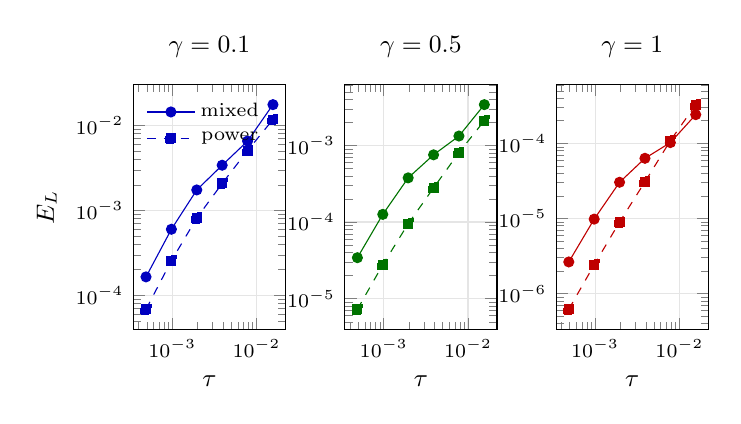
\begin{tikzpicture}
\begin{groupplot}[group style={group size=3 by 1,horizontal sep=0.75cm},
width=.29\textwidth,height=4.7cm,xmode=log,ymode=log,
grid=major,grid style={gray!20},tick label style={font=\scriptsize},
label style={font=\small},title style={font=\small},
legend style={font=\scriptsize,draw=none,fill=none},legend pos=north west]
\nextgroupplot[title={$\gamma=0.1$},xlabel={$\tau$},ylabel={$E_L$}]
\addplot[blue!75!black,mark=*,solid,mark size=1.8pt] coordinates {(0.00048828125,0.000164857997212) (0.0009765625,0.000599633045194) (0.001953125,0.00174248023572) (0.00390625,0.00340457824265) (0.0078125,0.00655620517347) (0.015625,0.0176068750324)};
\addlegendentry{mixed}
\addplot[blue!75!black,mark=square*,dashed,mark size=1.8pt] coordinates {(0.00048828125,6.85205523122e-05) (0.0009765625,0.000255176962409) (0.001953125,0.000813691543434) (0.00390625,0.00207656873155) (0.0078125,0.005061871412) (0.015625,0.0117639271822)};
\addlegendentry{power}
\nextgroupplot[title={$\gamma=0.5$},xlabel={$\tau$},ylabel={}]
\addplot[green!45!black,mark=*,solid,mark size=1.8pt] coordinates {(0.00048828125,3.42718836869e-05) (0.0009765625,0.000125993732926) (0.001953125,0.000377055144817) (0.00390625,0.000753532672574) (0.0078125,0.00132474504771) (0.015625,0.00340153756273)};
\addplot[green!45!black,mark=square*,dashed,mark size=1.8pt] coordinates {(0.00048828125,7.28444653717e-06) (0.0009765625,2.77275225218e-05) (0.001953125,9.48659891874e-05) (0.00390625,0.000278999095771) (0.0078125,0.000806004598041) (0.015625,0.00210354657997)};
\nextgroupplot[title={$\gamma=1$},xlabel={$\tau$},ylabel={}]
\addplot[red!75!black,mark=*,solid,mark size=1.8pt] coordinates {(0.00048828125,2.63644380706e-06) (0.0009765625,9.8015399975e-06) (0.001953125,3.03412276434e-05) (0.00390625,6.32343317342e-05) (0.0078125,0.000102333304607) (0.015625,0.000241024142508)};
\addplot[red!75!black,mark=square*,dashed,mark size=1.8pt] coordinates {(0.00048828125,6.18304485409e-07) (0.0009765625,2.41425690601e-06) (0.001953125,8.95639073115e-06) (0.00390625,3.07707315741e-05) (0.0078125,0.000108469290828) (0.015625,0.000327645540939)};
\end{groupplot}
\end{tikzpicture}
\caption{Maximum grid error for $N=8$, $K=32$. Each curve uses the
same initial datum and spatial cutoff throughout the refinement.
Faster convergence at fixed bandwidth is compatible with the rough-data
upper bound and does not establish its sharpness.}\label{fig:global}
\end{figure}

\subsection{The cubic remainder}
The local experiments use $N\in\{4,8,16,32\}$,
$\tau=N^{-3}$, and coefficients
$b_k=k^{-1/2-\gamma}e^{i\theta_k}$ for $1\leq k\leq N$.
The four phase choices are $\theta_k=0$ (even),
$\theta_k=-\pi/2$ (odd), $\theta_k=-\pi/2-\tau k^3/2$
(half Airy), and random angles with seed $518+N$.
After adding conjugate negative frequencies, rescale to
$\|f\|_{H^\gamma}=1$. The exact multiplier is summed through output
frequency $3N$, with its resonant part and its absolute Fourier
envelope retained separately.

Figure~\ref{fig:local} reports all 48 local cases. The normalized
remainder is bounded over the tested bandwidths. For half-Airy odd data,
the ratio of the $L^2$ remainder norm to the $L^2$ absolute-envelope norm
lies between $0.999962$ and $1.000000$. Thus these finite examples allow
almost coherent addition of Fourier terms. The proof uses the absolute
envelope and does not require cancellation of this type.
At total resonance, $\beta=-\alpha$ and
$\eta_\tau=1-\sinc^2(\tau\alpha/2)$, so the resonant remainder is
generally nonzero. The bounded finite sample does not establish a
uniform infinite-dimensional bound; Theorem~\ref{thm:local} does.

\begin{figure}[tb]
\centering
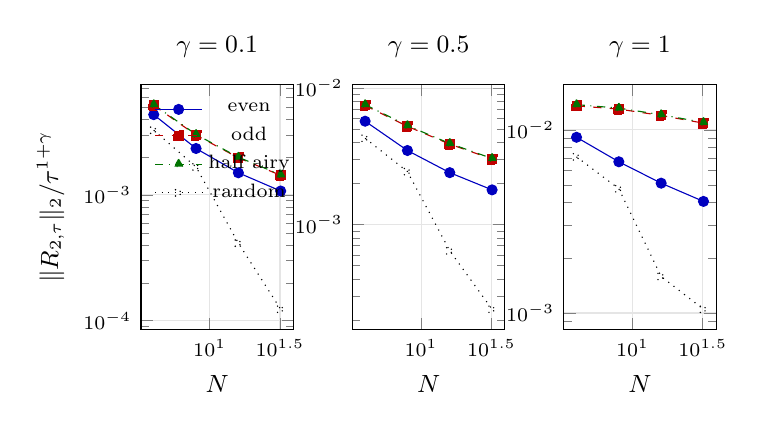
\begin{tikzpicture}
\begin{groupplot}[group style={group size=3 by 1,horizontal sep=0.75cm},
width=.29\textwidth,height=4.7cm,xmode=log,ymode=log,
grid=major,grid style={gray!20},tick label style={font=\scriptsize},
label style={font=\small},title style={font=\small},
legend style={font=\scriptsize,draw=none,fill=none},legend pos=north west]
\nextgroupplot[title={$\gamma=0.1$},xlabel={$N$},ylabel={$\|R_{2,\tau}\|_2/\tau^{1+\gamma}$}]
\addplot[blue!75!black,mark=*,solid,mark size=1.8pt] coordinates {(4,0.0043385048771) (8,0.00233658530004) (16,0.00149787174311) (32,0.00107330651685)};
\addlegendentry{even}
\addplot[red!75!black,mark=square*,dashed,mark size=1.8pt] coordinates {(4,0.00514384381352) (8,0.00298366747637) (16,0.00197183589325) (32,0.00142957289273)};
\addlegendentry{odd}
\addplot[green!45!black,mark=triangle*,dashdotted,mark size=1.8pt] coordinates {(4,0.00521022939043) (8,0.00301924167015) (16,0.00199298061448) (32,0.0014438740465)};
\addlegendentry{half airy}
\addplot[black,mark=x,dotted,mark size=1.8pt] coordinates {(4,0.00326143726086) (8,0.00166695298832) (16,0.000413806552389) (32,0.000123422993601)};
\addlegendentry{random}
\nextgroupplot[title={$\gamma=0.5$},xlabel={$N$},ylabel={}]
\addplot[blue!75!black,mark=*,solid,mark size=1.8pt] coordinates {(4,0.00572110324155) (8,0.00348923591339) (16,0.00240103839453) (32,0.00179560920995)};
\addplot[red!75!black,mark=square*,dashed,mark size=1.8pt] coordinates {(4,0.0074574724093) (8,0.00524296016038) (16,0.00388708237079) (32,0.0030196143849)};
\addplot[green!45!black,mark=triangle*,dashdotted,mark size=1.8pt] coordinates {(4,0.00756777887147) (8,0.00530981986784) (16,0.0039303786644) (32,0.00305059193252)};
\addplot[black,mark=x,dotted,mark size=1.8pt] coordinates {(4,0.00429186732411) (8,0.00244403551072) (16,0.000641984108951) (32,0.000239418984089)};
\nextgroupplot[title={$\gamma=1$},xlabel={$N$},ylabel={}]
\addplot[blue!75!black,mark=*,solid,mark size=1.8pt] coordinates {(4,0.00911900642753) (8,0.00669998319681) (16,0.00511796686746) (32,0.00406922646669)};
\addplot[red!75!black,mark=square*,dashed,mark size=1.8pt] coordinates {(4,0.0135386726082) (8,0.0130013987681) (16,0.0119933802803) (32,0.0108910688649)};
\addplot[green!45!black,mark=triangle*,dashdotted,mark size=1.8pt] coordinates {(4,0.0137477288927) (8,0.0131558979593) (16,0.0121107350395) (32,0.0109858737889)};
\addplot[black,mark=x,dotted,mark size=1.8pt] coordinates {(4,0.00712927153312) (8,0.0047703721466) (16,0.00158301967358) (32,0.00104770266775)};
\end{groupplot}
\end{tikzpicture}
\caption{The normalized full cubic remainder for four phase families,
$\|f\|_{H^\gamma}=1$ and $\tau=N^{-3}$. All output modes through $3N$
are included.}\label{fig:local}
\end{figure}

\subsection{Accumulation of defects and feedback}
For a fixed coarse step let $\Psi_\tau$ denote the implemented update
and let $r_n$ be the finer reference at $t_n$. Define
\[
d_n=r_{n+1}-\Psi_\tau(r_n),\qquad
g_n=\Psi_\tau(r_n)-\Psi_\tau(u_K^n)-S_\tau(r_n-u_K^n).
\]
The grid error $e_n=r_n-u_K^n$ therefore satisfies exactly
\[
S_{-t_m}e_m
 =\sum_{n=0}^{m-1}S_{-t_{n+1}}d_n
  +\sum_{n=0}^{m-1}S_{-t_{n+1}}g_n .
\]
The archives retain both sums and every individual Fourier defect and
feedback. The largest reconstruction discrepancy over all 48 global
runs is $3.93\cdot10^{-15}$. This identity is an accounting check on
the saved states, not an independent convergence estimate.

In the mixed $(\gamma,N,K,L)=(0.1,16,64,16)$ example,
the transported defect sum has coherence
$\|\sum S_{-t_{n+1}}d_n\|_2/\sum\|d_n\|_2=0.99448$
at $T$. The errors and the two accumulated components appear in
Figure~\ref{fig:defects}. At the peak error time, modes $k=\pm1$
contain $90.68\%$ of the error energy. Splitting each modal energy as
\[
|r_k-u_k|^2=(|r_k|-|u_k|)^2+
                 2|r_k||u_k|(1-\cos(\arg r_k-\arg u_k))
\]
gives a phase contribution of $99.83\%$ in that example.
The second summand is defined as zero when either magnitude is zero.
Across the 48 global runs, the phase fraction at peak ranges from
$86.48\%$ to $100.00\%$, whereas the fraction in modes $\pm1$ ranges
from $0.81\%$ to $96.77\%$. Low-mode concentration is therefore
case-dependent. The residual proof allows coherent accumulation and
does not assume statistically independent step errors.

\begin{figure}[tb]
\centering
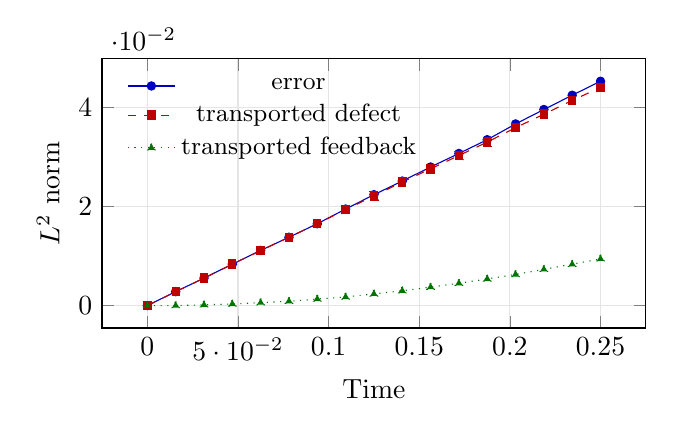
\begin{tikzpicture}
\begin{axis}[width=.70\textwidth,height=5cm,grid=major,grid style={gray!20},
xlabel={Time},ylabel={$L^2$ norm},legend pos=north west,
legend style={font=\small,draw=none,fill=none}]
\addplot[blue!75!black,mark=*,solid,mark size=1.5pt] coordinates {(0,0) (0.015625,0.00281766413354) (0.03125,0.00555380770827) (0.046875,0.00837507391698) (0.0625,0.0111517759578) (0.078125,0.0138159209597) (0.09375,0.0165452343666) (0.109375,0.0195174481608) (0.125,0.0224181452363) (0.140625,0.0251758458476) (0.15625,0.0280144099888) (0.171875,0.0307516630568) (0.1875,0.0335374792272) (0.203125,0.0367208787778) (0.21875,0.0396405905114) (0.234375,0.042528265304) (0.25,0.0453519355168)};
\addlegendentry{error}
\addplot[red!75!black,mark=square*,dashed,mark size=1.5pt] coordinates {(0,0) (0.015625,0.00281766413354) (0.03125,0.00554277180289) (0.046875,0.00837509273594) (0.0625,0.0111208177314) (0.078125,0.0138027906933) (0.09375,0.0165349421019) (0.109375,0.019389697921) (0.125,0.0221743668369) (0.140625,0.0249654468977) (0.15625,0.0276526987579) (0.171875,0.0303351037427) (0.1875,0.0330578079941) (0.203125,0.0359565569113) (0.21875,0.0386948168186) (0.234375,0.0414665002577) (0.25,0.0441085450375)};
\addlegendentry{transported defect}
\addplot[green!45!black,mark=triangle*,dotted,mark size=1.5pt] coordinates {(0,0) (0.015625,0) (0.03125,0.000152796228107) (0.046875,0.000329100546215) (0.0625,0.000591415771185) (0.078125,0.000881550615513) (0.09375,0.00132152950034) (0.109375,0.00174372429402) (0.125,0.00235902798342) (0.140625,0.00299673094885) (0.15625,0.00372559216201) (0.171875,0.0045097538091) (0.1875,0.00538491615705) (0.203125,0.0062934752615) (0.21875,0.00732868115906) (0.234375,0.0083564127375) (0.25,0.00944793548569)};
\addlegendentry{transported feedback}
\end{axis}\end{tikzpicture}
\caption{Error, transported defect sum, and transported feedback sum
for mixed data with $\gamma=0.1$, $N=16$, $K=64$, $L=16$.
The two components are vector sums and their norms are not additive.}
\label{fig:defects}
\end{figure}

The main campaign took 84.3 seconds and peaked at 390 MB resident memory
on the recorded single-thread local runtime. The accompanying submission
package contains this article and its editable source, the numerical
library, tests, scripts, seeds, configurations, compact scalar summaries
and vector figures. Its README gives installation, test and experiment
commands that regenerate all complex Fourier checkpoints, step defects
and reference comparisons. These generated arrays remain in the local
results directory and are excluded from version control.
The theorem concerns the exact time-semidiscrete update; a fully discrete
uniform convergence theorem and a rate lower bound are outside its scope.

\clearpage
\begin{thebibliography}{9}
\bibitem{LW}
B.~Li and Y.~Wu,
\emph{An Unfiltered Low-Regularity Integrator for the KdV Equation with Solutions Below $H^1$},
Foundations of Computational Mathematics \textbf{26} (2026), 1321--1380.
DOI: \href{https://doi.org/10.1007/s10208-025-09702-0}{10.1007/s10208-025-09702-0}.
The equation, lemma, and page references in this article use the 50-page author
manuscript at \url{https://www.polyu.edu.hk/ama/profile/byli/FoCM-3.pdf}.
\bibitem{BIT}
A.~V. Babin, A.~A. Ilyin and E.~S. Titi,
\emph{On the regularization mechanism for the periodic Korteweg--de Vries equation},
arXiv:0910.1389v2 (23 October 2010), \url{https://arxiv.org/abs/0910.1389v2}.
All theorem locators refer to this 42-page version.
\bibitem{AIM}
\texttt{MColbrook/AIM}, \emph{518. Removing the logarithmic loss in the Li--Wu KdV integrator},
fixed problem statement at commit
\texttt{c9929805cece044705abaaebe1cebddac1ba11a6} of \texttt{MColbrook/AIM}.
\bibitem{SCIPY}
The SciPy community, \emph{\texttt{scipy.integrate.solve\_ivp} documentation},
\url{https://docs.scipy.org/doc/scipy/reference/generated/scipy.integrate.solve_ivp.html},
accessed 10 October 2026.
\end{thebibliography}

\section*{AI use declaration}
ChatGPT was used to develop candidate arguments in the source research
conversation. Codex assisted with reconstructing that material, expanding
and auditing the natural-language proof, checking primary sources and
citation applicability, rewriting the manuscript, and implementing and
testing the numerical experiments. A separate fresh-context AI review
was used to look for mathematical and evidential objections. These
natural-language and computational checks do not constitute formal
verification or human peer review.
\end{document}
